\documentclass[1p]{elsarticle_modified}
%\bibliographystyle{elsarticle-num}

%\usepackage[colorlinks]{hyperref}
%\usepackage{abbrmath_seonhwa} %\Abb, \Ascr, \Acal ,\Abf, \Afrak
\usepackage{amsfonts}
\usepackage{amssymb}
\usepackage{amsmath}
\usepackage{amsthm}
\usepackage{scalefnt}
\usepackage{amsbsy}
\usepackage{kotex}
\usepackage{caption}
\usepackage{subfig}
\usepackage{color}
\usepackage{graphicx}
\usepackage{xcolor} %% white, black, red, green, blue, cyan, magenta, yellow
\usepackage{float}
\usepackage{setspace}
\usepackage{hyperref}

\usepackage{tikz}
\usetikzlibrary{arrows}

\usepackage{multirow}
\usepackage{array} % fixed length table
\usepackage{hhline}

%%%%%%%%%%%%%%%%%%%%%
\makeatletter
\renewcommand*\env@matrix[1][\arraystretch]{%
	\edef\arraystretch{#1}%
	\hskip -\arraycolsep
	\let\@ifnextchar\new@ifnextchar
	\array{*\c@MaxMatrixCols c}}
\makeatother %https://tex.stackexchange.com/questions/14071/how-can-i-increase-the-line-spacing-in-a-matrix
%%%%%%%%%%%%%%%

\usepackage[normalem]{ulem}

\newcommand{\msout}[1]{\ifmmode\text{\sout{\ensuremath{#1}}}\else\sout{#1}\fi}
%SOURCE: \msout is \stkout macro in https://tex.stackexchange.com/questions/20609/strikeout-in-math-mode

\newcommand{\cancel}[1]{
	\ifmmode
	{\color{red}\msout{#1}}
	\else
	{\color{red}\sout{#1}}
	\fi
}

\newcommand{\add}[1]{
	{\color{blue}\uwave{#1}}
}

\newcommand{\replace}[2]{
	\ifmmode
	{\color{red}\msout{#1}}{\color{blue}\uwave{#2}}
	\else
	{\color{red}\sout{#1}}{\color{blue}\uwave{#2}}
	\fi
}

\newcommand{\Sol}{\mathcal{S}} %segment
\newcommand{\D}{D} %diagram
\newcommand{\A}{\mathcal{A}} %arc


%%%%%%%%%%%%%%%%%%%%%%%%%%%%%5 test

\def\sl{\operatorname{\textup{SL}}(2,\Cbb)}
\def\psl{\operatorname{\textup{PSL}}(2,\Cbb)}
\def\quan{\mkern 1mu \triangleright \mkern 1mu}

\theoremstyle{definition}
\newtheorem{thm}{Theorem}[section]
\newtheorem{prop}[thm]{Proposition}
\newtheorem{lem}[thm]{Lemma}
\newtheorem{ques}[thm]{Question}
\newtheorem{cor}[thm]{Corollary}
\newtheorem{defn}[thm]{Definition}
\newtheorem{exam}[thm]{Example}
\newtheorem{rmk}[thm]{Remark}
\newtheorem{alg}[thm]{Algorithm}

\newcommand{\I}{\sqrt{-1}}
\begin{document}

%\begin{frontmatter}
%
%\title{Boundary parabolic representations of knots up to 8 crossings}
%
%%% Group authors per affiliation:
%\author{Yunhi Cho} 
%\address{Department of Mathematics, University of Seoul, Seoul, Korea}
%\ead{yhcho@uos.ac.kr}
%
%
%\author{Seonhwa Kim} %\fnref{s_kim}}
%\address{Center for Geometry and Physics, Institute for Basic Science, Pohang, 37673, Korea}
%\ead{ryeona17@ibs.re.kr}
%
%\author{Hyuk Kim}
%\address{Department of Mathematical Sciences, Seoul National University, Seoul 08826, Korea}
%\ead{hyukkim@snu.ac.kr}
%
%\author{Seokbeom Yoon}
%\address{Department of Mathematical Sciences, Seoul National University, Seoul, 08826,  Korea}
%\ead{sbyoon15@snu.ac.kr}
%
%\begin{abstract}
%We find all boundary parabolic representation of knots up to 8 crossings.
%
%\end{abstract}
%\begin{keyword}
%    \MSC[2010] 57M25 
%\end{keyword}
%
%\end{frontmatter}

%\linenumbers
%\tableofcontents
%
\newcommand\colored[1]{\textcolor{white}{\rule[-0.35ex]{0.8em}{1.4ex}}\kern-0.8em\color{red} #1}%
%\newcommand\colored[1]{\textcolor{white}{ #1}\kern-2.17ex	\textcolor{white}{ #1}\kern-1.81ex	\textcolor{white}{ #1}\kern-2.15ex\color{red}#1	}

{\Large $\underline{12n_{0634}~(K12n_{0634})}$}

\setlength{\tabcolsep}{10pt}
\renewcommand{\arraystretch}{1.6}
\vspace{1cm}\begin{tabular}{m{100pt}>{\centering\arraybackslash}m{274pt}}
\multirow{5}{120pt}{
	\centering
	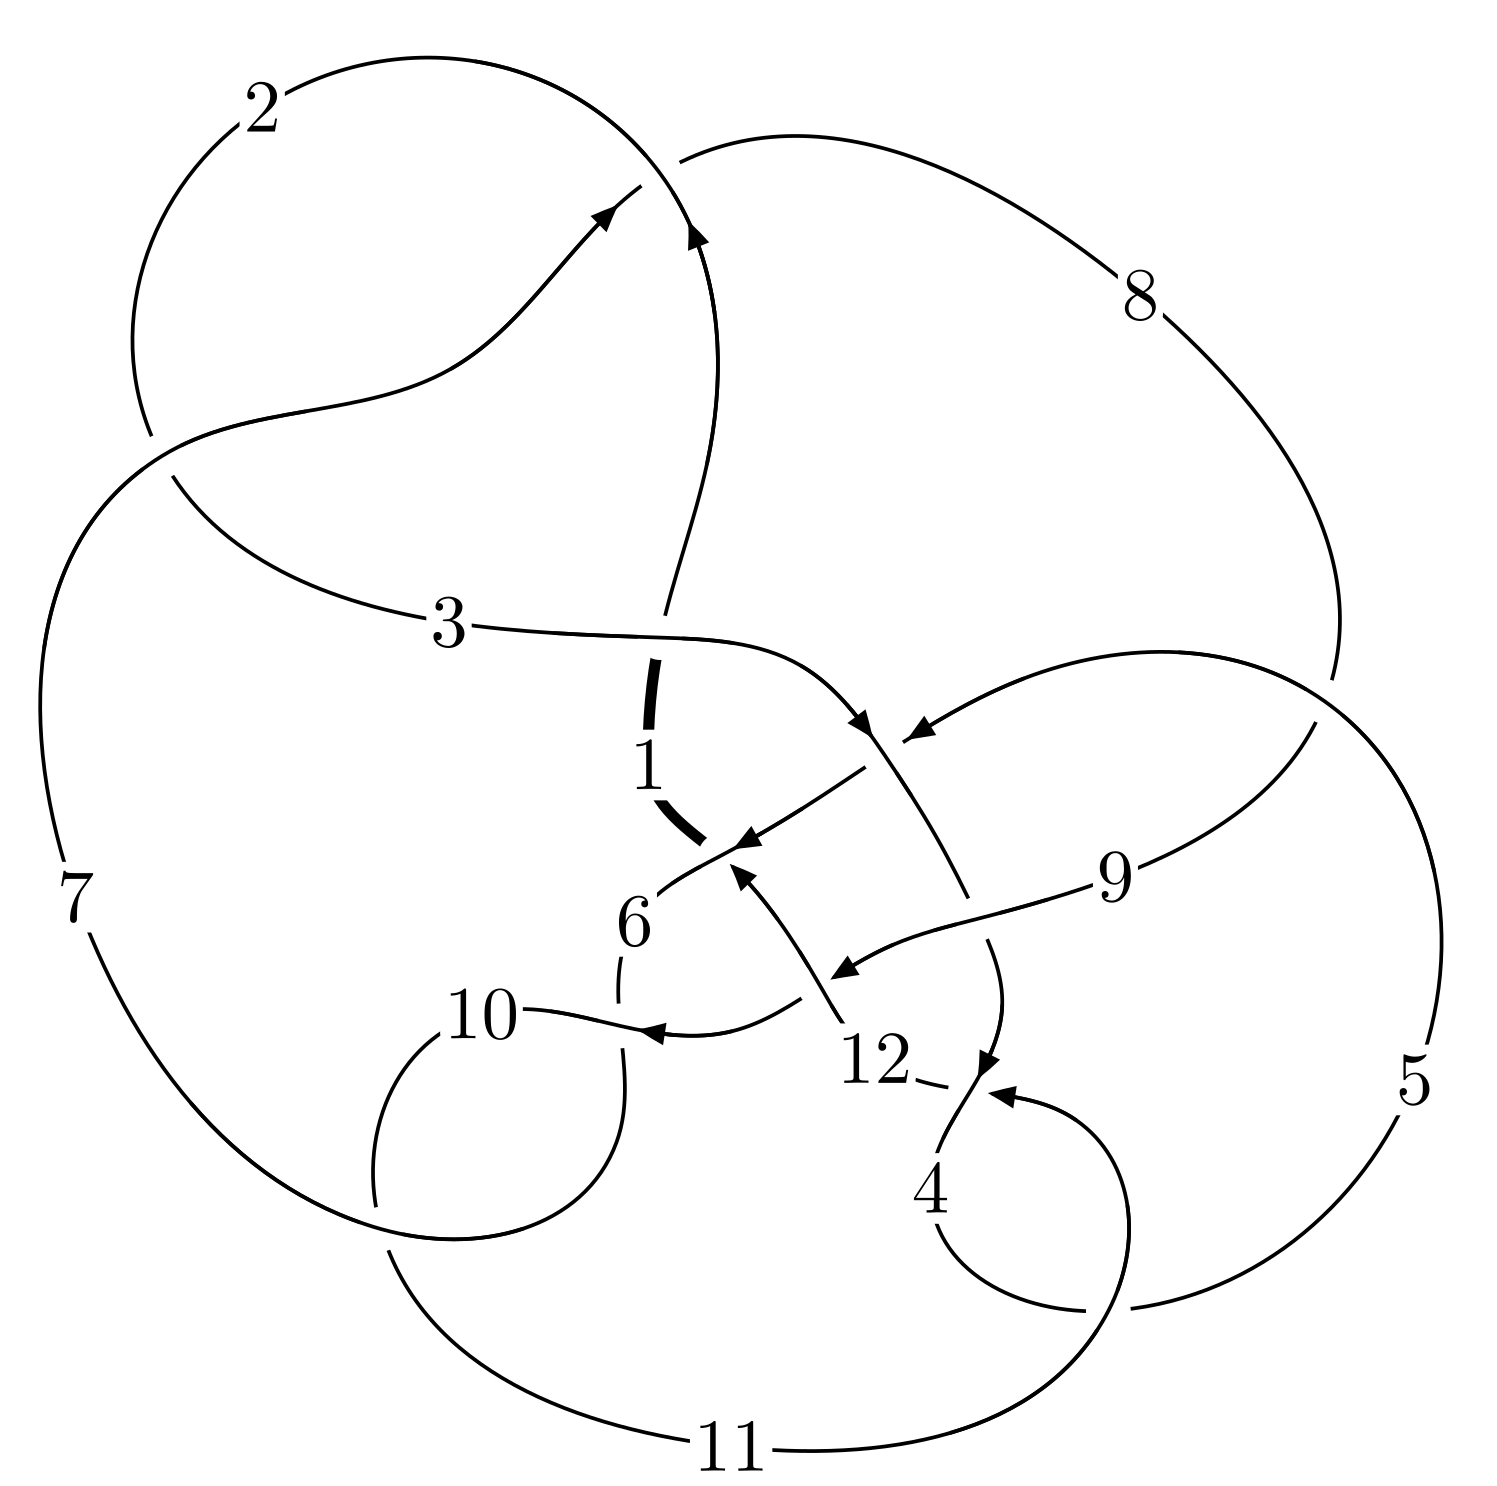
\includegraphics[width=112pt]{../../../GIT/diagram.site/Diagrams/png/2723_12n_0634.png}\\
\ \ \ A knot diagram\footnotemark}&
\allowdisplaybreaks
\textbf{Linearized knot diagam} \\
\cline{2-2}
 &
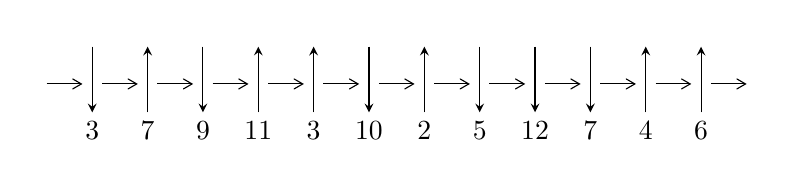
\begin{tikzpicture}[x=20pt, y=17pt]
	% nodes
	\node (C0) at (0, 0) {};
	\node (C1) at (1, 0) {};
	\node (C1U) at (1, +1) {};
	\node (C1D) at (1, -1) {3};

	\node (C2) at (2, 0) {};
	\node (C2U) at (2, +1) {};
	\node (C2D) at (2, -1) {7};

	\node (C3) at (3, 0) {};
	\node (C3U) at (3, +1) {};
	\node (C3D) at (3, -1) {9};

	\node (C4) at (4, 0) {};
	\node (C4U) at (4, +1) {};
	\node (C4D) at (4, -1) {11};

	\node (C5) at (5, 0) {};
	\node (C5U) at (5, +1) {};
	\node (C5D) at (5, -1) {3};

	\node (C6) at (6, 0) {};
	\node (C6U) at (6, +1) {};
	\node (C6D) at (6, -1) {10};

	\node (C7) at (7, 0) {};
	\node (C7U) at (7, +1) {};
	\node (C7D) at (7, -1) {2};

	\node (C8) at (8, 0) {};
	\node (C8U) at (8, +1) {};
	\node (C8D) at (8, -1) {5};

	\node (C9) at (9, 0) {};
	\node (C9U) at (9, +1) {};
	\node (C9D) at (9, -1) {12};

	\node (C10) at (10, 0) {};
	\node (C10U) at (10, +1) {};
	\node (C10D) at (10, -1) {7};

	\node (C11) at (11, 0) {};
	\node (C11U) at (11, +1) {};
	\node (C11D) at (11, -1) {4};

	\node (C12) at (12, 0) {};
	\node (C12U) at (12, +1) {};
	\node (C12D) at (12, -1) {6};
	\node (C13) at (13, 0) {};

	% arrows
	\draw[->,>={angle 60}]
	(C0) edge (C1) (C1) edge (C2) (C2) edge (C3) (C3) edge (C4) (C4) edge (C5) (C5) edge (C6) (C6) edge (C7) (C7) edge (C8) (C8) edge (C9) (C9) edge (C10) (C10) edge (C11) (C11) edge (C12) (C12) edge (C13) ;	\draw[->,>=stealth]
	(C1U) edge (C1D) (C2D) edge (C2U) (C3U) edge (C3D) (C4D) edge (C4U) (C5D) edge (C5U) (C6U) edge (C6D) (C7D) edge (C7U) (C8U) edge (C8D) (C9U) edge (C9D) (C10U) edge (C10D) (C11D) edge (C11U) (C12D) edge (C12U) ;
	\end{tikzpicture} \\
\hhline{~~} \\& 
\textbf{Solving Sequence} \\ \cline{2-2} 
 &
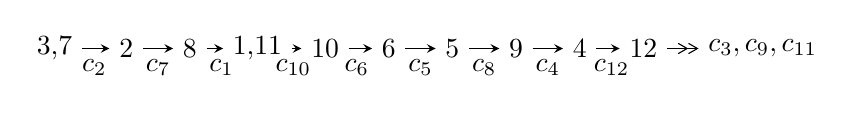
\begin{tikzpicture}[x=23pt, y=7pt]
	% node
	\node (A0) at (-1/8, 0) {3,7};
	\node (A1) at (1, 0) {2};
	\node (A2) at (2, 0) {8};
	\node (A3) at (49/16, 0) {1,11};
	\node (A4) at (33/8, 0) {10};
	\node (A5) at (41/8, 0) {6};
	\node (A6) at (49/8, 0) {5};
	\node (A7) at (57/8, 0) {9};
	\node (A8) at (65/8, 0) {4};
	\node (A9) at (73/8, 0) {12};
	\node (C1) at (1/2, -1) {$c_{2}$};
	\node (C2) at (3/2, -1) {$c_{7}$};
	\node (C3) at (5/2, -1) {$c_{1}$};
	\node (C4) at (29/8, -1) {$c_{10}$};
	\node (C5) at (37/8, -1) {$c_{6}$};
	\node (C6) at (45/8, -1) {$c_{5}$};
	\node (C7) at (53/8, -1) {$c_{8}$};
	\node (C8) at (61/8, -1) {$c_{4}$};
	\node (C9) at (69/8, -1) {$c_{12}$};
	\node (A10) at (11, 0) {$c_{3},c_{9},c_{11}$};

	% edge
	\draw[->,>=stealth]	
	(A0) edge (A1) (A1) edge (A2) (A2) edge (A3) (A3) edge (A4) (A4) edge (A5) (A5) edge (A6) (A6) edge (A7) (A7) edge (A8) (A8) edge (A9) ;
	\draw[->>,>={angle 60}]	
	(A9) edge (A10);
\end{tikzpicture} \\ 

\end{tabular} \\

\footnotetext{
The image of knot diagram is generated by the software ``\textbf{Draw programme}" developed by Andrew Bartholomew(\url{http://www.layer8.co.uk/maths/draw/index.htm\#Running-draw}), where we modified some parts for our purpose(\url{https://github.com/CATsTAILs/LinksPainter}).
}\phantom \\ \newline 
\centering \textbf{Ideals for irreducible components\footnotemark of $X_{\text{par}}$} 
 
\begin{align*}
I^u_{1}&=\langle 
-1.95711\times10^{172} u^{51}-3.47717\times10^{172} u^{50}+\cdots+1.87747\times10^{177} b+1.65522\times10^{176},\\
\phantom{I^u_{1}}&\phantom{= \langle  }5.80863\times10^{175} u^{51}+7.03687\times10^{175} u^{50}+\cdots+8.07312\times10^{178} a+1.92816\times10^{178},\\
\phantom{I^u_{1}}&\phantom{= \langle  }u^{52}+u^{51}+\cdots-430 u-1849\rangle \\
I^u_{2}&=\langle 
7.95354\times10^{18} u^{28}-2.49597\times10^{18} u^{27}+\cdots+1.30438\times10^{19} b+9.76819\times10^{18},\\
\phantom{I^u_{2}}&\phantom{= \langle  }-2.06470\times10^{19} u^{28}-4.89686\times10^{18} u^{27}+\cdots+1.30438\times10^{19} a-4.59506\times10^{19},\\
\phantom{I^u_{2}}&\phantom{= \langle  }u^{29}+16 u^{27}+\cdots+2 u+1\rangle \\
\\
\end{align*}
\raggedright * 2 irreducible components of $\dim_{\mathbb{C}}=0$, with total 81 representations.\\
\footnotetext{All coefficients of polynomials are rational numbers. But the coefficients are sometimes approximated in decimal forms when there is not enough margin.}
\newpage
\renewcommand{\arraystretch}{1}
\centering \section*{I. $I^u_{1}= \langle -1.96\times10^{172} u^{51}-3.48\times10^{172} u^{50}+\cdots+1.88\times10^{177} b+1.66\times10^{176},\;5.81\times10^{175} u^{51}+7.04\times10^{175} u^{50}+\cdots+8.07\times10^{178} a+1.93\times10^{178},\;u^{52}+u^{51}+\cdots-430 u-1849 \rangle$}
\flushleft \textbf{(i) Arc colorings}\\
\begin{tabular}{m{7pt} m{180pt} m{7pt} m{180pt} }
\flushright $a_{3}=$&$\begin{pmatrix}1\\0\end{pmatrix}$ \\
\flushright $a_{7}=$&$\begin{pmatrix}0\\u\end{pmatrix}$ \\
\flushright $a_{2}=$&$\begin{pmatrix}1\\u^2\end{pmatrix}$ \\
\flushright $a_{8}=$&$\begin{pmatrix}u\\u^3+u\end{pmatrix}$ \\
\flushright $a_{1}=$&$\begin{pmatrix}u^2+1\\u^2\end{pmatrix}$ \\
\flushright $a_{11}=$&$\begin{pmatrix}-0.000719502 u^{51}-0.000871642 u^{50}+\cdots-2.02990 u-0.238837\\0.0000104242 u^{51}+0.0000185205 u^{50}+\cdots-2.44475 u-0.0881622\end{pmatrix}$ \\
\flushright $a_{10}=$&$\begin{pmatrix}-0.000719502 u^{51}-0.000871642 u^{50}+\cdots-2.02990 u-0.238837\\-8.14632\times10^{-7} u^{51}-0.0000812325 u^{50}+\cdots-1.04897 u+0.193144\end{pmatrix}$ \\
\flushright $a_{6}=$&$\begin{pmatrix}0.000695591 u^{51}+0.000693094 u^{50}+\cdots+5.78811 u+1.78101\\0.000147181 u^{51}+0.000119151 u^{50}+\cdots+2.46237 u+0.340252\end{pmatrix}$ \\
\flushright $a_{5}=$&$\begin{pmatrix}0.000548410 u^{51}+0.000573943 u^{50}+\cdots+3.32574 u+1.44076\\0.000147181 u^{51}+0.000119151 u^{50}+\cdots+2.46237 u+0.340252\end{pmatrix}$ \\
\flushright $a_{9}=$&$\begin{pmatrix}-0.000562077 u^{51}-0.000571100 u^{50}+\cdots-6.77593 u-2.97489\\-0.000159864 u^{51}-0.000179227 u^{50}+\cdots-2.17934 u-0.533160\end{pmatrix}$ \\
\flushright $a_{4}=$&$\begin{pmatrix}0.000231771 u^{51}+0.000153448 u^{50}+\cdots+10.5786 u+4.67788\\0.0000301411 u^{51}+0.0000823394 u^{50}+\cdots+2.47373 u+0.457419\end{pmatrix}$ \\
\flushright $a_{12}=$&$\begin{pmatrix}0.000440440 u^{51}+0.000638660 u^{50}+\cdots-4.30838 u+4.57675\\0.0000737660 u^{51}+0.0000885300 u^{50}+\cdots-0.804093 u+0.949948\end{pmatrix}$\\&\end{tabular}
\flushleft \textbf{(ii) Obstruction class $= -1$}\\~\\
\flushleft \textbf{(iii) Cusp Shapes $= 0.000209766 u^{51}+0.000739361 u^{50}+\cdots+3.85584 u-4.14186$}\\~\\
\newpage\renewcommand{\arraystretch}{1}
\flushleft \textbf{(iv) u-Polynomials at the component}\newline \\
\begin{tabular}{m{50pt}|m{274pt}}
Crossings & \hspace{64pt}u-Polynomials at each crossing \\
\hline $$\begin{aligned}c_{1}\end{aligned}$$&$\begin{aligned}
&u^{52}+83 u^{51}+\cdots-10239762 u+3418801
\end{aligned}$\\
\hline $$\begin{aligned}c_{2},c_{7}\end{aligned}$$&$\begin{aligned}
&u^{52}- u^{51}+\cdots+430 u-1849
\end{aligned}$\\
\hline $$\begin{aligned}c_{3}\end{aligned}$$&$\begin{aligned}
&u^{52}- u^{51}+\cdots-96 u+9
\end{aligned}$\\
\hline $$\begin{aligned}c_{4},c_{11}\end{aligned}$$&$\begin{aligned}
&u^{52}-2 u^{51}+\cdots-1077 u-89
\end{aligned}$\\
\hline $$\begin{aligned}c_{5}\end{aligned}$$&$\begin{aligned}
&u^{52}+47 u^{50}+\cdots-950335 u-289973
\end{aligned}$\\
\hline $$\begin{aligned}c_{6},c_{10}\end{aligned}$$&$\begin{aligned}
&u^{52}+2 u^{51}+\cdots+91 u-181
\end{aligned}$\\
\hline $$\begin{aligned}c_{8}\end{aligned}$$&$\begin{aligned}
&u^{52}+5 u^{51}+\cdots-38226689 u+7428119
\end{aligned}$\\
\hline $$\begin{aligned}c_{9}\end{aligned}$$&$\begin{aligned}
&u^{52}-5 u^{51}+\cdots+324 u+356
\end{aligned}$\\
\hline $$\begin{aligned}c_{12}\end{aligned}$$&$\begin{aligned}
&u^{52}-2 u^{51}+\cdots-81165 u+4259
\end{aligned}$\\
\hline
\end{tabular}\\~\\
\newpage\renewcommand{\arraystretch}{1}
\flushleft \textbf{(v) Riley Polynomials at the component}\newline \\
\begin{tabular}{m{50pt}|m{274pt}}
Crossings & \hspace{64pt}Riley Polynomials at each crossing \\
\hline $$\begin{aligned}c_{1}\end{aligned}$$&$\begin{aligned}
&y^{52}-209 y^{51}+\cdots+1284466243376242 y+11688200277601
\end{aligned}$\\
\hline $$\begin{aligned}c_{2},c_{7}\end{aligned}$$&$\begin{aligned}
&y^{52}+83 y^{51}+\cdots-10239762 y+3418801
\end{aligned}$\\
\hline $$\begin{aligned}c_{3}\end{aligned}$$&$\begin{aligned}
&y^{52}-11 y^{51}+\cdots-4590 y+81
\end{aligned}$\\
\hline $$\begin{aligned}c_{4},c_{11}\end{aligned}$$&$\begin{aligned}
&y^{52}+50 y^{51}+\cdots-321727 y+7921
\end{aligned}$\\
\hline $$\begin{aligned}c_{5}\end{aligned}$$&$\begin{aligned}
&y^{52}+94 y^{51}+\cdots-346734679987 y+84084340729
\end{aligned}$\\
\hline $$\begin{aligned}c_{6},c_{10}\end{aligned}$$&$\begin{aligned}
&y^{52}-54 y^{51}+\cdots+1011111 y+32761
\end{aligned}$\\
\hline $$\begin{aligned}c_{8}\end{aligned}$$&$\begin{aligned}
&y^{52}-73 y^{51}+\cdots-308498524989461 y+55176951878161
\end{aligned}$\\
\hline $$\begin{aligned}c_{9}\end{aligned}$$&$\begin{aligned}
&y^{52}-25 y^{51}+\cdots+789296 y+126736
\end{aligned}$\\
\hline $$\begin{aligned}c_{12}\end{aligned}$$&$\begin{aligned}
&y^{52}+98 y^{51}+\cdots-7982256041 y+18139081
\end{aligned}$\\
\hline
\end{tabular}\\~\\
\newpage\flushleft \textbf{(vi) Complex Volumes and Cusp Shapes}
$$\begin{array}{c|c|c}  
\text{Solutions to }I^u_{1}& \I (\text{vol} + \sqrt{-1}CS) & \text{Cusp shape}\\
 \hline 
\begin{aligned}
u &= \phantom{-}0.275825 + 0.932345 I \\
a &= -0.380468 - 0.078038 I \\
b &= \phantom{-}1.52892 + 1.15015 I\end{aligned}
 & -2.42630 + 6.41308 I & \phantom{-}1.23938 - 7.68294 I \\ \hline\begin{aligned}
u &= \phantom{-}0.275825 - 0.932345 I \\
a &= -0.380468 + 0.078038 I \\
b &= \phantom{-}1.52892 - 1.15015 I\end{aligned}
 & -2.42630 - 6.41308 I & \phantom{-}1.23938 + 7.68294 I \\ \hline\begin{aligned}
u &= \phantom{-}0.539271 + 0.935679 I \\
a &= -0.287527 + 0.954049 I \\
b &= -0.817124 + 0.789515 I\end{aligned}
 & -3.75694 + 4.49624 I & -7.52077 - 6.70808 I \\ \hline\begin{aligned}
u &= \phantom{-}0.539271 - 0.935679 I \\
a &= -0.287527 - 0.954049 I \\
b &= -0.817124 - 0.789515 I\end{aligned}
 & -3.75694 - 4.49624 I & -7.52077 + 6.70808 I \\ \hline\begin{aligned}
u &= -0.650501 + 0.863107 I \\
a &= \phantom{-}0.691550 - 0.812723 I \\
b &= -1.61355 - 1.85935 I\end{aligned}
 & \phantom{-}0.50603 - 2.57474 I & \phantom{-0.000000 -}0. + 4.06110 I \\ \hline\begin{aligned}
u &= -0.650501 - 0.863107 I \\
a &= \phantom{-}0.691550 + 0.812723 I \\
b &= -1.61355 + 1.85935 I\end{aligned}
 & \phantom{-}0.50603 + 2.57474 I & \phantom{-0.000000 } 0. - 4.06110 I \\ \hline\begin{aligned}
u &= \phantom{-}0.202582 + 0.881244 I \\
a &= \phantom{-}0.630878 - 0.801031 I \\
b &= -0.512799 + 0.454432 I\end{aligned}
 & -1.81662 - 1.18879 I & -5.31113 + 2.20959 I \\ \hline\begin{aligned}
u &= \phantom{-}0.202582 - 0.881244 I \\
a &= \phantom{-}0.630878 + 0.801031 I \\
b &= -0.512799 - 0.454432 I\end{aligned}
 & -1.81662 + 1.18879 I & -5.31113 - 2.20959 I \\ \hline\begin{aligned}
u &= \phantom{-}0.351525 + 1.081680 I \\
a &= -0.672391 + 1.023130 I \\
b &= -0.217102 - 0.172805 I\end{aligned}
 & -8.65330 - 1.89169 I & -8.34506 + 0.93318 I \\ \hline\begin{aligned}
u &= \phantom{-}0.351525 - 1.081680 I \\
a &= -0.672391 - 1.023130 I \\
b &= -0.217102 + 0.172805 I\end{aligned}
 & -8.65330 + 1.89169 I & -8.34506 - 0.93318 I\\
 \hline 
 \end{array}$$\newpage$$\begin{array}{c|c|c}  
\text{Solutions to }I^u_{1}& \I (\text{vol} + \sqrt{-1}CS) & \text{Cusp shape}\\
 \hline 
\begin{aligned}
u &= -0.818940 + 0.160767 I \\
a &= -1.69144 + 0.20465 I \\
b &= -0.928736 + 0.671508 I\end{aligned}
 & -5.38897 + 0.87571 I & -2.85912 + 2.34335 I \\ \hline\begin{aligned}
u &= -0.818940 - 0.160767 I \\
a &= -1.69144 - 0.20465 I \\
b &= -0.928736 - 0.671508 I\end{aligned}
 & -5.38897 - 0.87571 I & -2.85912 - 2.34335 I \\ \hline\begin{aligned}
u &= -0.335509 + 0.751647 I \\
a &= \phantom{-}0.538199 - 0.371856 I \\
b &= -0.932426 - 0.178983 I\end{aligned}
 & -0.27804 - 1.89990 I & \phantom{-}0.73245 + 4.61007 I \\ \hline\begin{aligned}
u &= -0.335509 - 0.751647 I \\
a &= \phantom{-}0.538199 + 0.371856 I \\
b &= -0.932426 + 0.178983 I\end{aligned}
 & -0.27804 + 1.89990 I & \phantom{-}0.73245 - 4.61007 I \\ \hline\begin{aligned}
u &= \phantom{-}0.213597 + 1.222440 I \\
a &= -0.743596 - 0.589889 I \\
b &= \phantom{-}1.60989 - 1.34032 I\end{aligned}
 & \phantom{-}1.01333 + 1.02881 I & \phantom{-0.000000 } 0 \\ \hline\begin{aligned}
u &= \phantom{-}0.213597 - 1.222440 I \\
a &= -0.743596 + 0.589889 I \\
b &= \phantom{-}1.60989 + 1.34032 I\end{aligned}
 & \phantom{-}1.01333 - 1.02881 I & \phantom{-0.000000 } 0 \\ \hline\begin{aligned}
u &= -0.055615 + 0.755904 I \\
a &= \phantom{-}0.49398 - 1.42299 I \\
b &= -1.190970 - 0.372066 I\end{aligned}
 & -2.79971 - 1.53838 I & -4.05410 + 0.44087 I \\ \hline\begin{aligned}
u &= -0.055615 - 0.755904 I \\
a &= \phantom{-}0.49398 + 1.42299 I \\
b &= -1.190970 + 0.372066 I\end{aligned}
 & -2.79971 + 1.53838 I & -4.05410 - 0.44087 I \\ \hline\begin{aligned}
u &= \phantom{-}0.679978\phantom{ +0.000000I} \\
a &= \phantom{-}1.52551\phantom{ +0.000000I} \\
b &= \phantom{-}0.501507\phantom{ +0.000000I}\end{aligned}
 & -1.67869\phantom{ +0.000000I} & -6.69150\phantom{ +0.000000I} \\ \hline\begin{aligned}
u &= \phantom{-}0.336439 + 0.585453 I \\
a &= -0.443953 - 0.493321 I \\
b &= -0.599232 - 0.191514 I\end{aligned}
 & -3.82874 - 0.83282 I & -6.69897 - 1.25074 I\\
 \hline 
 \end{array}$$\newpage$$\begin{array}{c|c|c}  
\text{Solutions to }I^u_{1}& \I (\text{vol} + \sqrt{-1}CS) & \text{Cusp shape}\\
 \hline 
\begin{aligned}
u &= \phantom{-}0.336439 - 0.585453 I \\
a &= -0.443953 + 0.493321 I \\
b &= -0.599232 + 0.191514 I\end{aligned}
 & -3.82874 + 0.83282 I & -6.69897 + 1.25074 I \\ \hline\begin{aligned}
u &= \phantom{-}0.521240 + 0.365317 I \\
a &= \phantom{-}0.555831 + 0.734286 I \\
b &= -1.084070 + 0.405815 I\end{aligned}
 & -1.16726 - 3.02767 I & \phantom{-}1.89586 + 2.76037 I \\ \hline\begin{aligned}
u &= \phantom{-}0.521240 - 0.365317 I \\
a &= \phantom{-}0.555831 - 0.734286 I \\
b &= -1.084070 - 0.405815 I\end{aligned}
 & -1.16726 + 3.02767 I & \phantom{-}1.89586 - 2.76037 I \\ \hline\begin{aligned}
u &= -0.898610 + 1.083740 I \\
a &= -0.832366 - 0.553360 I \\
b &= -0.203830 + 0.717311 I\end{aligned}
 & -7.83351 + 4.08846 I & \phantom{-0.000000 } 0 \\ \hline\begin{aligned}
u &= -0.898610 - 1.083740 I \\
a &= -0.832366 + 0.553360 I \\
b &= -0.203830 - 0.717311 I\end{aligned}
 & -7.83351 - 4.08846 I & \phantom{-0.000000 } 0 \\ \hline\begin{aligned}
u &= \phantom{-}1.02788 + 1.21603 I \\
a &= \phantom{-}0.666350 - 1.075790 I \\
b &= \phantom{-}2.88476 + 0.58421 I\end{aligned}
 & -9.81716 - 1.76389 I & \phantom{-0.000000 } 0 \\ \hline\begin{aligned}
u &= \phantom{-}1.02788 - 1.21603 I \\
a &= \phantom{-}0.666350 + 1.075790 I \\
b &= \phantom{-}2.88476 - 0.58421 I\end{aligned}
 & -9.81716 + 1.76389 I & \phantom{-0.000000 } 0 \\ \hline\begin{aligned}
u &= -0.08564 + 1.59213 I \\
a &= -0.412998 + 0.094265 I \\
b &= \phantom{-}0.692278 + 0.084135 I\end{aligned}
 & -8.51191 - 3.22667 I & \phantom{-0.000000 } 0 \\ \hline\begin{aligned}
u &= -0.08564 - 1.59213 I \\
a &= -0.412998 - 0.094265 I \\
b &= \phantom{-}0.692278 - 0.084135 I\end{aligned}
 & -8.51191 + 3.22667 I & \phantom{-0.000000 } 0 \\ \hline\begin{aligned}
u &= -0.330077 + 0.195063 I \\
a &= \phantom{-}0.625921 + 0.929420 I \\
b &= \phantom{-}0.680678 - 0.511018 I\end{aligned}
 & \phantom{-}1.12780 - 0.87427 I & \phantom{-}7.10299 + 3.37562 I\\
 \hline 
 \end{array}$$\newpage$$\begin{array}{c|c|c}  
\text{Solutions to }I^u_{1}& \I (\text{vol} + \sqrt{-1}CS) & \text{Cusp shape}\\
 \hline 
\begin{aligned}
u &= -0.330077 - 0.195063 I \\
a &= \phantom{-}0.625921 - 0.929420 I \\
b &= \phantom{-}0.680678 + 0.511018 I\end{aligned}
 & \phantom{-}1.12780 + 0.87427 I & \phantom{-}7.10299 - 3.37562 I \\ \hline\begin{aligned}
u &= \phantom{-}0.255114 + 0.232956 I \\
a &= -3.71521 + 1.79997 I \\
b &= -0.880754 - 0.179713 I\end{aligned}
 & -5.75128 - 6.56432 I & -4.11138 + 4.05271 I \\ \hline\begin{aligned}
u &= \phantom{-}0.255114 - 0.232956 I \\
a &= -3.71521 - 1.79997 I \\
b &= -0.880754 + 0.179713 I\end{aligned}
 & -5.75128 + 6.56432 I & -4.11138 - 4.05271 I \\ \hline\begin{aligned}
u &= -0.337796\phantom{ +0.000000I} \\
a &= \phantom{-}3.69732\phantom{ +0.000000I} \\
b &= \phantom{-}1.37016\phantom{ +0.000000I}\end{aligned}
 & -0.727216\phantom{ +0.000000I} & -13.1080\phantom{ +0.000000I} \\ \hline\begin{aligned}
u &= \phantom{-}0.03672 + 1.74560 I \\
a &= -0.251249 + 0.023127 I \\
b &= \phantom{-}1.289730 + 0.212055 I\end{aligned}
 & -12.39400 + 0.81454 I & \phantom{-0.000000 } 0 \\ \hline\begin{aligned}
u &= \phantom{-}0.03672 - 1.74560 I \\
a &= -0.251249 - 0.023127 I \\
b &= \phantom{-}1.289730 - 0.212055 I\end{aligned}
 & -12.39400 - 0.81454 I & \phantom{-0.000000 } 0 \\ \hline\begin{aligned}
u &= -1.15761 + 1.51843 I \\
a &= \phantom{-}0.586482 + 0.796448 I \\
b &= \phantom{-}2.30536 - 1.24673 I\end{aligned}
 & -10.15170 - 6.43419 I & \phantom{-0.000000 } 0 \\ \hline\begin{aligned}
u &= -1.15761 - 1.51843 I \\
a &= \phantom{-}0.586482 - 0.796448 I \\
b &= \phantom{-}2.30536 + 1.24673 I\end{aligned}
 & -10.15170 + 6.43419 I & \phantom{-0.000000 } 0 \\ \hline\begin{aligned}
u &= \phantom{-}0.32226 + 1.90220 I \\
a &= \phantom{-}0.014803 - 0.900992 I \\
b &= \phantom{-}1.44976 + 0.57133 I\end{aligned}
 & -19.1346 + 2.1490 I & \phantom{-0.000000 } 0 \\ \hline\begin{aligned}
u &= \phantom{-}0.32226 - 1.90220 I \\
a &= \phantom{-}0.014803 + 0.900992 I \\
b &= \phantom{-}1.44976 - 0.57133 I\end{aligned}
 & -19.1346 - 2.1490 I & \phantom{-0.000000 } 0\\
 \hline 
 \end{array}$$\newpage$$\begin{array}{c|c|c}  
\text{Solutions to }I^u_{1}& \I (\text{vol} + \sqrt{-1}CS) & \text{Cusp shape}\\
 \hline 
\begin{aligned}
u &= \phantom{-}0.07800 + 1.98796 I \\
a &= -0.109017 - 0.866405 I \\
b &= \phantom{-}0.805068 + 0.656452 I\end{aligned}
 & -15.4556 + 6.9522 I & \phantom{-0.000000 } 0 \\ \hline\begin{aligned}
u &= \phantom{-}0.07800 - 1.98796 I \\
a &= -0.109017 + 0.866405 I \\
b &= \phantom{-}0.805068 - 0.656452 I\end{aligned}
 & -15.4556 - 6.9522 I & \phantom{-0.000000 } 0 \\ \hline\begin{aligned}
u &= -0.02112 + 2.09350 I \\
a &= -0.144533 + 0.825946 I \\
b &= \phantom{-}0.865609 - 1.012250 I\end{aligned}
 & -14.6985 - 0.9884 I & \phantom{-0.000000 } 0 \\ \hline\begin{aligned}
u &= -0.02112 - 2.09350 I \\
a &= -0.144533 - 0.825946 I \\
b &= \phantom{-}0.865609 + 1.012250 I\end{aligned}
 & -14.6985 + 0.9884 I & \phantom{-0.000000 } 0 \\ \hline\begin{aligned}
u &= \phantom{-}0.53139 + 2.03050 I \\
a &= \phantom{-}0.245255 + 0.983595 I \\
b &= -3.40407 - 0.93661 I\end{aligned}
 & \phantom{-}19.4506 + 5.7616 I & \phantom{-0.000000 } 0 \\ \hline\begin{aligned}
u &= \phantom{-}0.53139 - 2.03050 I \\
a &= \phantom{-}0.245255 - 0.983595 I \\
b &= -3.40407 + 0.93661 I\end{aligned}
 & \phantom{-}19.4506 - 5.7616 I & \phantom{-0.000000 } 0 \\ \hline\begin{aligned}
u &= -0.43024 + 2.08016 I \\
a &= \phantom{-}0.185917 - 0.896546 I \\
b &= -2.73017 + 0.92922 I\end{aligned}
 & \phantom{-}17.8356 - 14.3502 I & \phantom{-0.000000 } 0 \\ \hline\begin{aligned}
u &= -0.43024 - 2.08016 I \\
a &= \phantom{-}0.185917 + 0.896546 I \\
b &= -2.73017 - 0.92922 I\end{aligned}
 & \phantom{-}17.8356 + 14.3502 I & \phantom{-0.000000 } 0 \\ \hline\begin{aligned}
u &= -0.09944 + 2.16592 I \\
a &= \phantom{-}0.924083 + 0.081345 I \\
b &= -3.92522 - 0.71460 I\end{aligned}
 & -15.4081 + 4.9026 I & \phantom{-0.000000 } 0 \\ \hline\begin{aligned}
u &= -0.09944 - 2.16592 I \\
a &= \phantom{-}0.924083 - 0.081345 I \\
b &= -3.92522 + 0.71460 I\end{aligned}
 & -15.4081 - 4.9026 I & \phantom{-0.000000 } 0\\
 \hline 
 \end{array}$$\newpage$$\begin{array}{c|c|c}  
\text{Solutions to }I^u_{1}& \I (\text{vol} + \sqrt{-1}CS) & \text{Cusp shape}\\
 \hline 
\begin{aligned}
u &= -0.47962 + 2.20629 I \\
a &= \phantom{-}0.053614 + 0.744727 I \\
b &= \phantom{-}1.49215 - 0.97274 I\end{aligned}
 & -18.5854 - 3.5520 I & \phantom{-0.000000 } 0 \\ \hline\begin{aligned}
u &= -0.47962 - 2.20629 I \\
a &= \phantom{-}0.053614 - 0.744727 I \\
b &= \phantom{-}1.49215 + 0.97274 I\end{aligned}
 & -18.5854 + 3.5520 I & \phantom{-0.000000 } 0\\
 \hline 
 \end{array}$$\newpage\newpage\renewcommand{\arraystretch}{1}
\centering \section*{II. $I^u_{2}= \langle 7.95\times10^{18} u^{28}-2.50\times10^{18} u^{27}+\cdots+1.30\times10^{19} b+9.77\times10^{18},\;-2.06\times10^{19} u^{28}-4.90\times10^{18} u^{27}+\cdots+1.30\times10^{19} a-4.60\times10^{19},\;u^{29}+16 u^{27}+\cdots+2 u+1 \rangle$}
\flushleft \textbf{(i) Arc colorings}\\
\begin{tabular}{m{7pt} m{180pt} m{7pt} m{180pt} }
\flushright $a_{3}=$&$\begin{pmatrix}1\\0\end{pmatrix}$ \\
\flushright $a_{7}=$&$\begin{pmatrix}0\\u\end{pmatrix}$ \\
\flushright $a_{2}=$&$\begin{pmatrix}1\\u^2\end{pmatrix}$ \\
\flushright $a_{8}=$&$\begin{pmatrix}u\\u^3+u\end{pmatrix}$ \\
\flushright $a_{1}=$&$\begin{pmatrix}u^2+1\\u^2\end{pmatrix}$ \\
\flushright $a_{11}=$&$\begin{pmatrix}1.58289 u^{28}+0.375416 u^{27}+\cdots+23.0341 u+3.52278\\-0.609755 u^{28}+0.191352 u^{27}+\cdots-1.62838 u-0.748874\end{pmatrix}$ \\
\flushright $a_{10}=$&$\begin{pmatrix}1.58289 u^{28}+0.375416 u^{27}+\cdots+23.0341 u+3.52278\\-0.646274 u^{28}+0.321379 u^{27}+\cdots+0.705339 u-0.373458\end{pmatrix}$ \\
\flushright $a_{6}=$&$\begin{pmatrix}-2.19231 u^{28}-0.581219 u^{27}+\cdots-25.5255 u-3.87277\\0.146160 u^{28}+0.168172 u^{27}+\cdots-3.05911 u+0.0131335\end{pmatrix}$ \\
\flushright $a_{5}=$&$\begin{pmatrix}-2.33847 u^{28}-0.749392 u^{27}+\cdots-22.4664 u-3.88591\\0.146160 u^{28}+0.168172 u^{27}+\cdots-3.05911 u+0.0131335\end{pmatrix}$ \\
\flushright $a_{9}=$&$\begin{pmatrix}1.23953 u^{28}+0.189431 u^{27}+\cdots-8.70535 u-5.08357\\0.592887 u^{28}+0.289661 u^{27}+\cdots+7.84451 u+1.80937\end{pmatrix}$ \\
\flushright $a_{4}=$&$\begin{pmatrix}-3.39570 u^{28}-0.362303 u^{27}+\cdots-20.3142 u+1.55184\\0.716281 u^{28}+0.0775215 u^{27}+\cdots-1.88678 u-0.0652422\end{pmatrix}$ \\
\flushright $a_{12}=$&$\begin{pmatrix}1.88363 u^{28}-0.861725 u^{27}+\cdots-12.0156 u-6.82950\\-0.288048 u^{28}+0.0864079 u^{27}+\cdots-1.05603 u-1.20804\end{pmatrix}$\\&\end{tabular}
\flushleft \textbf{(ii) Obstruction class $= 1$}\\~\\
\flushleft \textbf{(iii) Cusp Shapes $= -\frac{37295273734905786033}{13043842048949049407} u^{28}+\frac{7379073912415012035}{13043842048949049407} u^{27}+\cdots+\frac{523698604375136567}{13043842048949049407} u-\frac{12328496894734939546}{13043842048949049407}$}\\~\\
\newpage\renewcommand{\arraystretch}{1}
\flushleft \textbf{(iv) u-Polynomials at the component}\newline \\
\begin{tabular}{m{50pt}|m{274pt}}
Crossings & \hspace{64pt}u-Polynomials at each crossing \\
\hline $$\begin{aligned}c_{1}\end{aligned}$$&$\begin{aligned}
&u^{29}-32 u^{28}+\cdots-30 u+1
\end{aligned}$\\
\hline $$\begin{aligned}c_{2}\end{aligned}$$&$\begin{aligned}
&u^{29}+16 u^{27}+\cdots+2 u+1
\end{aligned}$\\
\hline $$\begin{aligned}c_{3}\end{aligned}$$&$\begin{aligned}
&u^{29}- u^{27}+\cdots+4 u+1
\end{aligned}$\\
\hline $$\begin{aligned}c_{4}\end{aligned}$$&$\begin{aligned}
&u^{29}+u^{28}+\cdots- u-13
\end{aligned}$\\
\hline $$\begin{aligned}c_{5}\end{aligned}$$&$\begin{aligned}
&u^{29}+u^{28}+\cdots- u-1
\end{aligned}$\\
\hline $$\begin{aligned}c_{6}\end{aligned}$$&$\begin{aligned}
&u^{29}+u^{28}+\cdots-3 u-1
\end{aligned}$\\
\hline $$\begin{aligned}c_{7}\end{aligned}$$&$\begin{aligned}
&u^{29}+16 u^{27}+\cdots+2 u-1
\end{aligned}$\\
\hline $$\begin{aligned}c_{8}\end{aligned}$$&$\begin{aligned}
&u^{29}-6 u^{27}+\cdots+5 u+1
\end{aligned}$\\
\hline $$\begin{aligned}c_{9}\end{aligned}$$&$\begin{aligned}
&u^{29}-4 u^{28}+\cdots+24 u-4
\end{aligned}$\\
\hline $$\begin{aligned}c_{10}\end{aligned}$$&$\begin{aligned}
&u^{29}- u^{28}+\cdots-3 u+1
\end{aligned}$\\
\hline $$\begin{aligned}c_{11}\end{aligned}$$&$\begin{aligned}
&u^{29}- u^{28}+\cdots- u+13
\end{aligned}$\\
\hline $$\begin{aligned}c_{12}\end{aligned}$$&$\begin{aligned}
&u^{29}- u^{28}+\cdots+355 u+187
\end{aligned}$\\
\hline
\end{tabular}\\~\\
\newpage\renewcommand{\arraystretch}{1}
\flushleft \textbf{(v) Riley Polynomials at the component}\newline \\
\begin{tabular}{m{50pt}|m{274pt}}
Crossings & \hspace{64pt}Riley Polynomials at each crossing \\
\hline $$\begin{aligned}c_{1}\end{aligned}$$&$\begin{aligned}
&y^{29}-52 y^{28}+\cdots+34 y-1
\end{aligned}$\\
\hline $$\begin{aligned}c_{2},c_{7}\end{aligned}$$&$\begin{aligned}
&y^{29}+32 y^{28}+\cdots-30 y-1
\end{aligned}$\\
\hline $$\begin{aligned}c_{3}\end{aligned}$$&$\begin{aligned}
&y^{29}-2 y^{28}+\cdots+26 y-1
\end{aligned}$\\
\hline $$\begin{aligned}c_{4},c_{11}\end{aligned}$$&$\begin{aligned}
&y^{29}+23 y^{28}+\cdots-2209 y-169
\end{aligned}$\\
\hline $$\begin{aligned}c_{5}\end{aligned}$$&$\begin{aligned}
&y^{29}+15 y^{28}+\cdots+11 y-1
\end{aligned}$\\
\hline $$\begin{aligned}c_{6},c_{10}\end{aligned}$$&$\begin{aligned}
&y^{29}-17 y^{28}+\cdots+17 y-1
\end{aligned}$\\
\hline $$\begin{aligned}c_{8}\end{aligned}$$&$\begin{aligned}
&y^{29}-12 y^{28}+\cdots-103 y-1
\end{aligned}$\\
\hline $$\begin{aligned}c_{9}\end{aligned}$$&$\begin{aligned}
&y^{29}-8 y^{28}+\cdots-288 y-16
\end{aligned}$\\
\hline $$\begin{aligned}c_{12}\end{aligned}$$&$\begin{aligned}
&y^{29}+39 y^{28}+\cdots+65437 y-34969
\end{aligned}$\\
\hline
\end{tabular}\\~\\
\newpage\flushleft \textbf{(vi) Complex Volumes and Cusp Shapes}
$$\begin{array}{c|c|c}  
\text{Solutions to }I^u_{2}& \I (\text{vol} + \sqrt{-1}CS) & \text{Cusp shape}\\
 \hline 
\begin{aligned}
u &= -0.501818 + 0.833839 I \\
a &= \phantom{-}0.467030 + 0.518760 I \\
b &= -1.186310 - 0.660678 I\end{aligned}
 & -2.46701 + 3.31089 I & -6.64762 - 4.28533 I \\ \hline\begin{aligned}
u &= -0.501818 - 0.833839 I \\
a &= \phantom{-}0.467030 - 0.518760 I \\
b &= -1.186310 + 0.660678 I\end{aligned}
 & -2.46701 - 3.31089 I & -6.64762 + 4.28533 I \\ \hline\begin{aligned}
u &= \phantom{-}0.395046 + 0.881302 I \\
a &= \phantom{-}0.193357 - 1.331450 I \\
b &= \phantom{-}1.139830 + 0.271865 I\end{aligned}
 & -6.12414 + 8.00905 I & -5.12519 - 8.45010 I \\ \hline\begin{aligned}
u &= \phantom{-}0.395046 - 0.881302 I \\
a &= \phantom{-}0.193357 + 1.331450 I \\
b &= \phantom{-}1.139830 - 0.271865 I\end{aligned}
 & -6.12414 - 8.00905 I & -5.12519 + 8.45010 I \\ \hline\begin{aligned}
u &= -0.341041 + 1.028870 I \\
a &= -0.194038 - 0.579843 I \\
b &= \phantom{-}1.10689 - 1.28067 I\end{aligned}
 & -3.12004 - 6.46709 I & -9.74691 + 8.24915 I \\ \hline\begin{aligned}
u &= -0.341041 - 1.028870 I \\
a &= -0.194038 + 0.579843 I \\
b &= \phantom{-}1.10689 + 1.28067 I\end{aligned}
 & -3.12004 + 6.46709 I & -9.74691 - 8.24915 I \\ \hline\begin{aligned}
u &= \phantom{-}0.400082 + 1.085830 I \\
a &= \phantom{-}0.741612 + 0.558186 I \\
b &= -1.54514 + 1.73471 I\end{aligned}
 & \phantom{-}1.43870 + 1.55601 I & \phantom{-}3.91538 - 4.80433 I \\ \hline\begin{aligned}
u &= \phantom{-}0.400082 - 1.085830 I \\
a &= \phantom{-}0.741612 - 0.558186 I \\
b &= -1.54514 - 1.73471 I\end{aligned}
 & \phantom{-}1.43870 - 1.55601 I & \phantom{-}3.91538 + 4.80433 I \\ \hline\begin{aligned}
u &= -0.377353 + 1.105050 I \\
a &= \phantom{-}0.019943 - 0.931023 I \\
b &= -1.48812 - 0.50305 I\end{aligned}
 & -3.06298 - 3.21483 I & -6.22465 + 3.26026 I \\ \hline\begin{aligned}
u &= -0.377353 - 1.105050 I \\
a &= \phantom{-}0.019943 + 0.931023 I \\
b &= -1.48812 + 0.50305 I\end{aligned}
 & -3.06298 + 3.21483 I & -6.22465 - 3.26026 I\\
 \hline 
 \end{array}$$\newpage$$\begin{array}{c|c|c}  
\text{Solutions to }I^u_{2}& \I (\text{vol} + \sqrt{-1}CS) & \text{Cusp shape}\\
 \hline 
\begin{aligned}
u &= -0.757913 + 0.894886 I \\
a &= -0.934300 + 0.874778 I \\
b &= \phantom{-}1.59792 + 2.38337 I\end{aligned}
 & -0.51479 - 2.85047 I & -6.69492 + 4.19394 I \\ \hline\begin{aligned}
u &= -0.757913 - 0.894886 I \\
a &= -0.934300 - 0.874778 I \\
b &= \phantom{-}1.59792 - 2.38337 I\end{aligned}
 & -0.51479 + 2.85047 I & -6.69492 - 4.19394 I \\ \hline\begin{aligned}
u &= \phantom{-}0.284256 + 1.182870 I \\
a &= \phantom{-}0.333089 - 0.615425 I \\
b &= -1.232700 + 0.271698 I\end{aligned}
 & -2.12362 + 0.73935 I & -5.54663 - 2.17801 I \\ \hline\begin{aligned}
u &= \phantom{-}0.284256 - 1.182870 I \\
a &= \phantom{-}0.333089 + 0.615425 I \\
b &= -1.232700 - 0.271698 I\end{aligned}
 & -2.12362 - 0.73935 I & -5.54663 + 2.17801 I \\ \hline\begin{aligned}
u &= \phantom{-}0.125391 + 0.740741 I \\
a &= \phantom{-}0.072781 + 1.150700 I \\
b &= \phantom{-}0.445959 + 0.328062 I\end{aligned}
 & -0.218621 + 1.074110 I & -0.75381 - 2.66974 I \\ \hline\begin{aligned}
u &= \phantom{-}0.125391 - 0.740741 I \\
a &= \phantom{-}0.072781 - 1.150700 I \\
b &= \phantom{-}0.445959 - 0.328062 I\end{aligned}
 & -0.218621 - 1.074110 I & -0.75381 + 2.66974 I \\ \hline\begin{aligned}
u &= \phantom{-}0.856142 + 1.047000 I \\
a &= -0.906222 + 0.682310 I \\
b &= -0.823807 - 0.830433 I\end{aligned}
 & -6.75266 - 3.66088 I & -3.57875 + 1.97522 I \\ \hline\begin{aligned}
u &= \phantom{-}0.856142 - 1.047000 I \\
a &= -0.906222 - 0.682310 I \\
b &= -0.823807 + 0.830433 I\end{aligned}
 & -6.75266 + 3.66088 I & -3.57875 - 1.97522 I \\ \hline\begin{aligned}
u &= -0.09611 + 1.48953 I \\
a &= \phantom{-}0.207292 - 0.225440 I \\
b &= \phantom{-}0.209690 + 0.379206 I\end{aligned}
 & -9.07326 - 3.27525 I & -11.96737 + 3.20156 I \\ \hline\begin{aligned}
u &= -0.09611 - 1.48953 I \\
a &= \phantom{-}0.207292 + 0.225440 I \\
b &= \phantom{-}0.209690 - 0.379206 I\end{aligned}
 & -9.07326 + 3.27525 I & -11.96737 - 3.20156 I\\
 \hline 
 \end{array}$$\newpage$$\begin{array}{c|c|c}  
\text{Solutions to }I^u_{2}& \I (\text{vol} + \sqrt{-1}CS) & \text{Cusp shape}\\
 \hline 
\begin{aligned}
u &= -0.464529\phantom{ +0.000000I} \\
a &= \phantom{-}2.40413\phantom{ +0.000000I} \\
b &= \phantom{-}1.14153\phantom{ +0.000000I}\end{aligned}
 & -0.233389\phantom{ +0.000000I} & \phantom{-}4.21310\phantom{ +0.000000I} \\ \hline\begin{aligned}
u &= -0.162389 + 0.372510 I \\
a &= \phantom{-}1.81490 + 1.30389 I \\
b &= -1.027750 + 0.895148 I\end{aligned}
 & -4.36963 + 2.21765 I & -9.43891 - 3.55386 I \\ \hline\begin{aligned}
u &= -0.162389 - 0.372510 I \\
a &= \phantom{-}1.81490 - 1.30389 I \\
b &= -1.027750 - 0.895148 I\end{aligned}
 & -4.36963 - 2.21765 I & -9.43891 + 3.55386 I \\ \hline\begin{aligned}
u &= \phantom{-}0.120647 + 0.309845 I \\
a &= -2.64004 + 2.81826 I \\
b &= \phantom{-}0.376943 + 0.344347 I\end{aligned}
 & -5.97746 - 1.81572 I & -6.79885 + 3.34834 I \\ \hline\begin{aligned}
u &= \phantom{-}0.120647 - 0.309845 I \\
a &= -2.64004 - 2.81826 I \\
b &= \phantom{-}0.376943 - 0.344347 I\end{aligned}
 & -5.97746 + 1.81572 I & -6.79885 - 3.34834 I \\ \hline\begin{aligned}
u &= -0.08118 + 1.72162 I \\
a &= -0.376707 - 0.332059 I \\
b &= \phantom{-}1.30625 + 0.74373 I\end{aligned}
 & -12.44300 + 1.68015 I & -8.40294 + 0. I\phantom{ +0.000000I} \\ \hline\begin{aligned}
u &= -0.08118 - 1.72162 I \\
a &= -0.376707 + 0.332059 I \\
b &= \phantom{-}1.30625 - 0.74373 I\end{aligned}
 & -12.44300 - 1.68015 I & -8.40294 + 0. I\phantom{ +0.000000I} \\ \hline\begin{aligned}
u &= \phantom{-}0.36851 + 2.08278 I \\
a &= -0.000762 - 0.835761 I \\
b &= \phantom{-}1.54959 + 0.95102 I\end{aligned}
 & -17.4518 + 2.8402 I & \phantom{-0.000000 } 0 \\ \hline\begin{aligned}
u &= \phantom{-}0.36851 - 2.08278 I \\
a &= -0.000762 + 0.835761 I \\
b &= \phantom{-}1.54959 - 0.95102 I\end{aligned}
 & -17.4518 - 2.8402 I & \phantom{-0.000000 } 0\\
 \hline 
 \end{array}$$\newpage
\newpage\renewcommand{\arraystretch}{1}
\centering \section*{ III. u-Polynomials}
\begin{tabular}{m{50pt}|m{274pt}}
Crossings & \hspace{64pt}u-Polynomials at each crossing \\
\hline $$\begin{aligned}c_{1}\end{aligned}$$&$\begin{aligned}
&(u^{29}-32 u^{28}+\cdots-30 u+1)\\
&\cdot(u^{52}+83 u^{51}+\cdots-10239762 u+3418801)
\end{aligned}$\\
\hline $$\begin{aligned}c_{2}\end{aligned}$$&$\begin{aligned}
&(u^{29}+16 u^{27}+\cdots+2 u+1)(u^{52}- u^{51}+\cdots+430 u-1849)
\end{aligned}$\\
\hline $$\begin{aligned}c_{3}\end{aligned}$$&$\begin{aligned}
&(u^{29}- u^{27}+\cdots+4 u+1)(u^{52}- u^{51}+\cdots-96 u+9)
\end{aligned}$\\
\hline $$\begin{aligned}c_{4}\end{aligned}$$&$\begin{aligned}
&(u^{29}+u^{28}+\cdots- u-13)(u^{52}-2 u^{51}+\cdots-1077 u-89)
\end{aligned}$\\
\hline $$\begin{aligned}c_{5}\end{aligned}$$&$\begin{aligned}
&(u^{29}+u^{28}+\cdots- u-1)(u^{52}+47 u^{50}+\cdots-950335 u-289973)
\end{aligned}$\\
\hline $$\begin{aligned}c_{6}\end{aligned}$$&$\begin{aligned}
&(u^{29}+u^{28}+\cdots-3 u-1)(u^{52}+2 u^{51}+\cdots+91 u-181)
\end{aligned}$\\
\hline $$\begin{aligned}c_{7}\end{aligned}$$&$\begin{aligned}
&(u^{29}+16 u^{27}+\cdots+2 u-1)(u^{52}- u^{51}+\cdots+430 u-1849)
\end{aligned}$\\
\hline $$\begin{aligned}c_{8}\end{aligned}$$&$\begin{aligned}
&(u^{29}-6 u^{27}+\cdots+5 u+1)(u^{52}+5 u^{51}+\cdots-3.82267\times10^{7} u+7428119)
\end{aligned}$\\
\hline $$\begin{aligned}c_{9}\end{aligned}$$&$\begin{aligned}
&(u^{29}-4 u^{28}+\cdots+24 u-4)(u^{52}-5 u^{51}+\cdots+324 u+356)
\end{aligned}$\\
\hline $$\begin{aligned}c_{10}\end{aligned}$$&$\begin{aligned}
&(u^{29}- u^{28}+\cdots-3 u+1)(u^{52}+2 u^{51}+\cdots+91 u-181)
\end{aligned}$\\
\hline $$\begin{aligned}c_{11}\end{aligned}$$&$\begin{aligned}
&(u^{29}- u^{28}+\cdots- u+13)(u^{52}-2 u^{51}+\cdots-1077 u-89)
\end{aligned}$\\
\hline $$\begin{aligned}c_{12}\end{aligned}$$&$\begin{aligned}
&(u^{29}- u^{28}+\cdots+355 u+187)(u^{52}-2 u^{51}+\cdots-81165 u+4259)
\end{aligned}$\\
\hline
\end{tabular}\newpage\renewcommand{\arraystretch}{1}
\centering \section*{ IV. Riley Polynomials}
\begin{tabular}{m{50pt}|m{274pt}}
Crossings & \hspace{64pt}Riley Polynomials at each crossing \\
\hline $$\begin{aligned}c_{1}\end{aligned}$$&$\begin{aligned}
&(y^{29}-52 y^{28}+\cdots+34 y-1)\\
&\cdot(y^{52}-209 y^{51}+\cdots+1284466243376242 y+11688200277601)
\end{aligned}$\\
\hline $$\begin{aligned}c_{2},c_{7}\end{aligned}$$&$\begin{aligned}
&(y^{29}+32 y^{28}+\cdots-30 y-1)\\
&\cdot(y^{52}+83 y^{51}+\cdots-10239762 y+3418801)
\end{aligned}$\\
\hline $$\begin{aligned}c_{3}\end{aligned}$$&$\begin{aligned}
&(y^{29}-2 y^{28}+\cdots+26 y-1)(y^{52}-11 y^{51}+\cdots-4590 y+81)
\end{aligned}$\\
\hline $$\begin{aligned}c_{4},c_{11}\end{aligned}$$&$\begin{aligned}
&(y^{29}+23 y^{28}+\cdots-2209 y-169)\\
&\cdot(y^{52}+50 y^{51}+\cdots-321727 y+7921)
\end{aligned}$\\
\hline $$\begin{aligned}c_{5}\end{aligned}$$&$\begin{aligned}
&(y^{29}+15 y^{28}+\cdots+11 y-1)\\
&\cdot(y^{52}+94 y^{51}+\cdots-346734679987 y+84084340729)
\end{aligned}$\\
\hline $$\begin{aligned}c_{6},c_{10}\end{aligned}$$&$\begin{aligned}
&(y^{29}-17 y^{28}+\cdots+17 y-1)(y^{52}-54 y^{51}+\cdots+1011111 y+32761)
\end{aligned}$\\
\hline $$\begin{aligned}c_{8}\end{aligned}$$&$\begin{aligned}
&(y^{29}-12 y^{28}+\cdots-103 y-1)\\
&\cdot(y^{52}-73 y^{51}+\cdots-308498524989461 y+55176951878161)
\end{aligned}$\\
\hline $$\begin{aligned}c_{9}\end{aligned}$$&$\begin{aligned}
&(y^{29}-8 y^{28}+\cdots-288 y-16)\\
&\cdot(y^{52}-25 y^{51}+\cdots+789296 y+126736)
\end{aligned}$\\
\hline $$\begin{aligned}c_{12}\end{aligned}$$&$\begin{aligned}
&(y^{29}+39 y^{28}+\cdots+65437 y-34969)\\
&\cdot(y^{52}+98 y^{51}+\cdots-7982256041 y+18139081)
\end{aligned}$\\
\hline
\end{tabular}
\vskip 2pc
\end{document}